\documentclass{article}
\usepackage{PreambleCommon}
\usepackage{minted}


\title{Assignment 6: Heaps and Trees \\[5pt] Part 1: Heaps \\[8pt] CS3305/W01 Data Structures}
\author{Casey Hampson}

\begin{document}
\maketitle


\section*{Program Output}

\begin{center}
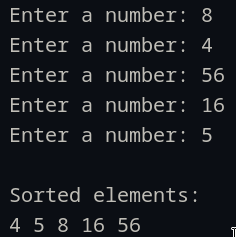
\includegraphics[width=0.4\linewidth]{res/1.png}
\end{center}


\section*{Changes Needed}
Since I didn't just copy/paste the listing in the book (I changed some style and added/removed comments for my own personal clarity), I wanted to just write the (three) changes I made to convert it to a MIN heap.

In the \mintinline{java}|AddObject()| method for a MAX heap, we would test if the current node is larger than its parent, in which case we swap the two. This is done with the \mintinline{java}|compareTo()| function, which returns a positive result if the first element is larger than the second. For our MIN heap, we want to do the opposite: if the current node is \textit{less} than its parent, we do the swap. Since the \mintinline{java}|compareTo()| function returns a negative result if the first argument is less than its parent, all we need to do is swap the comparator in the if statement.

Similar logic applies to the \mintinline{java}|RemoveRoot()| method. Instead of testing for if the children are larger than one another and if the current node is larger than its largest child, we look for if the children are smaller than one another and if the current node is smaller than its smallest child, which involves a switching of the comparator in the if statements.



\pagebreak
\section*{Source Code}
\inputminted{java}{./P1.java}




\end{document}
